\RequirePackage{ifpdf}
%\documentclass[journal]{vgtc}                % final (journal style)
\documentclass[review,journal]{vgtc}         % review (journal style)
%\documentclass[widereview]{vgtc}             % wide-spaced review
%\documentclass[preprint,journal]{vgtc}       % preprint (journal style)
%\documentclass[electronic,journal]{vgtc}     % electronic version, journal

%% Uncomment one of the lines above depending on where your paper is
%% in the conference process. ``review'' and ``widereview'' are for review
%% submission, ``preprint'' is for pre-publication, and the final version
%% doesn't use a specific qualifier. Further, ``electronic'' includes
%% hyperreferences for more convenient online viewing.

%% Please use one of the ``review'' options in combination with the
%% assigned online id (see below) ONLY if your paper uses a double blind
%% review process. Some conferences, like IEEE Vis and InfoVis, have NOT
%% in the past.

%% Please note that the use of figures other than the optional teaser is not permitted on the first page
%% of the journal version.  Figures should begin on the second page and be
%% in CMYK or Grey scale format, otherwise, colour shifting may occur
%% during the printing process.  Papers submitted with figures other than the optional teaser on the
%% first page will be refused.
%\begin{figure}[htb]
%	\centering
%	\fbox{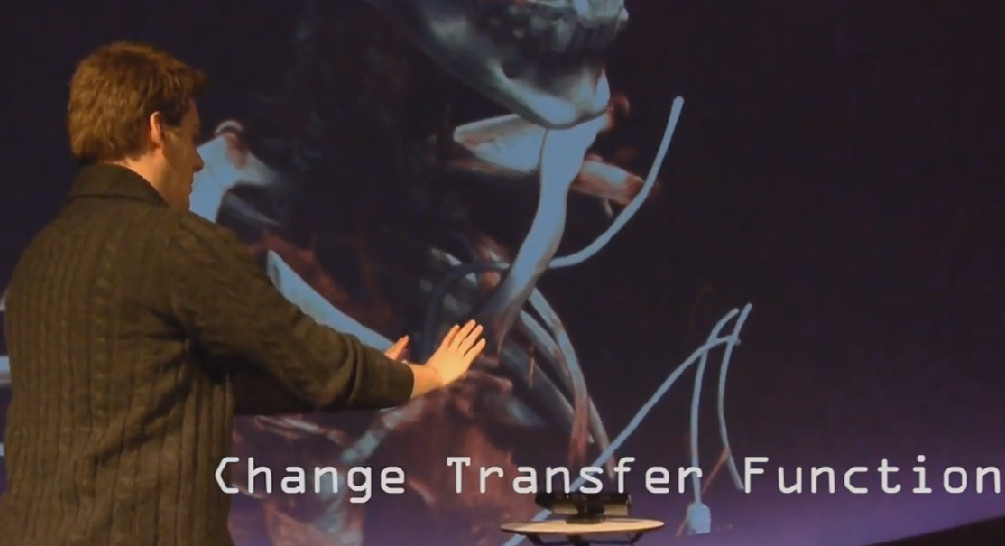
\includegraphics[width=1.0\linewidth]{images/dome_tf_change}}
%	\caption{Dome Closeup}
%	\label{img:dome_tf_change}
%\end{figure}

%% These three lines bring in essential packages: ``mathptmx'' for Type 1
%% typefaces, ``graphicx'' for inclusion of EPS figures. and ``times''
%% for proper handling of the times font family.

\usepackage{mathptmx}
\usepackage{graphicx}
\usepackage{times}
\usepackage{amsmath}
\usepackage{flushend}
\usepackage{subfigure}
\usepackage[noabbrev]{cleveref}
%\usepackage[caption=false]{subfig}
\setlength{\fboxsep}{0pt}
\newcommand{\todo}[1]{\textbf{\textcolor{red}{[TODO: {#1}]}}}

%% We encourage the use of mathptmx for consistent usage of times font
%% throughout the proceedings. However, if you encounter conflicts
%% with other math-related packages, you may want to disable it.

%% This turns references into clickable hyperlinks.
%%\usepackage[bookmarks,backref=true,linkcolor=black]{hyperref} %,colorlinks
%%\hypersetup{
%%  pdfauthor = {},
%%  pdftitle = {},
%%  pdfsubject = {},
%%  pdfkeywords = {},
%%  colorlinks=true,
%%  linkcolor= black,
%%  citecolor= black,
%%  pageanchor=true,
%%  urlcolor = black,
%%  plainpages = false,
%%  linktocpage
%%}

%% If you are submitting a paper to a conference for review with a double
%% blind reviewing process, please replace the value ``0'' below with your
%% OnlineID. Otherwise, you may safely leave it at ``0''.
\onlineid{0}

%% declare the category of your paper, only shown in review mode
\vgtccategory{Position Paper}

%% allow for this line if you want the electronic option to work properly
\vgtcinsertpkg

%% In preprint mode you may define your own headline.
%\preprinttext{To appear in an IEEE VGTC sponsored conference.}

%% Paper title.

\title{Hands-only 2D vs 3D interaction for scientific data exploration in a user vs viewer perspective}

%% This is how authors are specified in the journal style

%% indicate IEEE Member or Student Member in form indicated below
%% indicate IEEE Member or Student Member in form indicated below
\author{Erik Sund\'en, \textit{Member, IEEE} and Timo Ropinski, \textit{Member, IEEE}}
\authorfooter{
%% insert punctuation at end of each item
\item
 Erik Sund\'en and Timo Ropinski are with Link{\"o}ping University. E-mail: \{erik.sunden,timo.ropinski\}@liu.se.
}


%other entries to be set up for journal
\shortauthortitle{Sund\'en \MakeLowercase{\textit{et al.}}: Hands-only 2D vs 3D interaction when exploring volume data}
%\shortauthortitle{Firstauthor \MakeLowercase{\textit{et al.}}: Paper Title}

%% Abstract section.
\abstract{
In this paper we share our experiences with 2D and 3D interaction in different scenarios and environments which involve not only a user, but a certain amount of additional viewers, with different level of expertise in the area of volume exploration. Our additional focus is on hands-only interaction which based on previous work is a very natural form of interacting with the data. We can conclude, that good interaction in our scenarios could benefit from a focus on the user, instead of the viewer. While some natural exploratory interaction methods fit well for the user, they may be less beneficial for the actual viewers, and vice versa. Of course, an appropriate natural interaction for the user can in many scenarios be an appropriate interaction for the viewers, but our findings show that it usually highly dependent on the setting where the interaction and viewing takes place.
} % end of abstract

%% Keywords that describe your work. Will show as 'Index Terms' in journal
%% please capitalize first letter and insert punctuation after last keyword
\keywords{interaction, volume data, touch display, kinect}

%% ACM Computing Classification System (CCS). 
%% See <http://www.acm.org/class/1998/> for details.
%% The ``\CCScat'' command takes four arguments.

%\CCScatlist{ % not used in journal version
%   \CCScat{I.3.7}{Computer Graphics}{Three-Dimensional Graphics and Realism}{Color, shading, shadowing, and texture}
%}

%% Uncomment below to include a teaser figure.
%  \teaser{
%  \centering
%  \includegraphics[width=16cm]{CypressView}
%  \caption{In the Clouds: Vancouver from Cypress Mountain.}
%  }

%% Uncomment below to disable the manuscript note
%\renewcommand{\manuscriptnotetxt}{}

%% Copyright space is enabled by default as required by guidelines.
%% It is disabled by the 'review' option or via the following command:
% \nocopyrightspace

%%%%%%%%%%%%%%%%%%%%%%%%%%%%%%%%%%%%%%%%%%%%%%%%%%%%%%%%%%%%%%%%
%%%%%%%%%%%%%%%%%%%%%% START OF THE PAPER %%%%%%%%%%%%%%%%%%%%%%
%%%%%%%%%%%%%%%%%%%%%%%%%%%%%%%%%%%%%%%%%%%%%%%%%%%%%%%%%%%%%%%%%

\begin{document}

%% the only exception to this rule is the \firstsection command
%\firstsection{Introduction}\label{sec:introduction}

%% The ``\maketitle'' command must be the first command after the
%% ``\begin{document}'' command. It prepares and prints the title block.
\maketitle

\section{Introduction}\label{sec:introduction}

A common way to classify the use of visualization is to divide it into exploration, analysis and presentation. 
Each usecase typically requires a different approach and tools. 
While the exploration phase requires a flexible interaction with the visualization, 
the presentation phase is scaled down to allow the user to change only a few parameters or use a pre-determined animation. 
This distinction has to our knowledge not been done for interaction, where it is more common to refer to the level of expertise of the user. 
This manuscript will focus on the use of interaction for presentation. 
This involves one or more people interacting with a visualization in order to present information to an audience that may consist of a single person or many people. 

While we comment on expert viewers, the focus this paper is on none expert viewers, together with either an expert or none expert user. Our definition of expert is a person which is familiar within the area of volume data exploration.

....Touchless 3D interaction (kinect) vs touch screen 2D interaction....different scenarios such as slicing, clipping, zooming in 2D and 3D visualization of medical volume data.

\section{Why Hands-only?}

Using an object such as a mouse, can be useful both in 2D and 3D movements.

If the user has training with a certain device coupled with a specific application, the expert user may certainly benefit from the type of interaction instead of hands-only interaction.

However, for a none expert, which is the focus of this paper, a mouse/joystick offers unnatural ways of exploring the scientific data, as the hands are not directly interacting with the visualization of the data.

Mouse vs Kinect \cite{doi:10.1117/12.2006994}

Natural of touchless \cite{O'hara:2013:NTP:2442106.2442111}

Volume Cracker (3D interaction with gadgets) \cite{Laha:2013:VCB:2491367.2491368}

\section{2D Touch Interaction}

Position Paper Touch Interaction \cite{isenberg:hal-00781512}

Importance of Touch \cite{Robles-De-La-Torre:2006:IST:1158827.1159097}

Direct Touch Interaction Volume Exploration \cite{Klein:2012:DSD:2322389.2322403}

Autopsy Table \cite{LRFPY11}

\section{3D Touchless Interaction}

Kinect dicom \cite{zora82163}

Kinect operation \cite{OHaraGSPVMCCRDC14}

Interactive Slice WIM \cite{Coffey:2012:ISW:2360744.2360843}

Touchless surgery \cite{Mentis:2012:IPI:2207676.2208536}

Touching the 3rd dimension \cite{DBLP:journals/dagstuhl-reports/KeefeKSR12}

\section{Gestures}

Evaluation of Gesture \cite{Kirmizibayrak:2011:EGB:2087756.2087764}

Discuss gesture vs postures \cite{isenberg:hal-00781237} for kinect, and gesture available for both touch and kinect.

\section{(Daniel) Scenario: Single user exploration}

This scenario deals the situation when the presentation is performed on a small screen, such as a tablet or desktop monitor, and the audience consists of a few people. 
The distance between the audience and the presenter is typically small and allows for a tight communication between the two parts. 
The audience can easily communicate preferences in what to explore and may in some cases even intervene with the presenter to interact with the visualization. 
An intuitive interaction can therefore engage the audience and create a more dynamic presentation.
An example can be seen in~\cref{img:touch_workstation}, where the presenter uses a touch screen to interact with a fetus scanned using ultrasound.
The presenter can in this case switch to different modes, which controls the behaviour of the gestures. 
The standard mode rotates, translates and zooms using single finger, two fingers moving together and pinching, respectively. 
Switching to transfer function mode will change the interpretation of the single finger touch such that the threshold and opacity are changed according to the horizontal and vertical movement.

%This scenario deals with small screens and 
%User-centered...
%
%Mouse can be relevant, as touch devices.
%
%Touch good, reaching to the data. Especially when the user in question is not an expert in handling connected devices in that specific scenario.
%
%Clipping, 2D to 3D representation of region.
%
%Rotation, gripping points.

\begin{figure}[htb]
	\centering
	\fbox{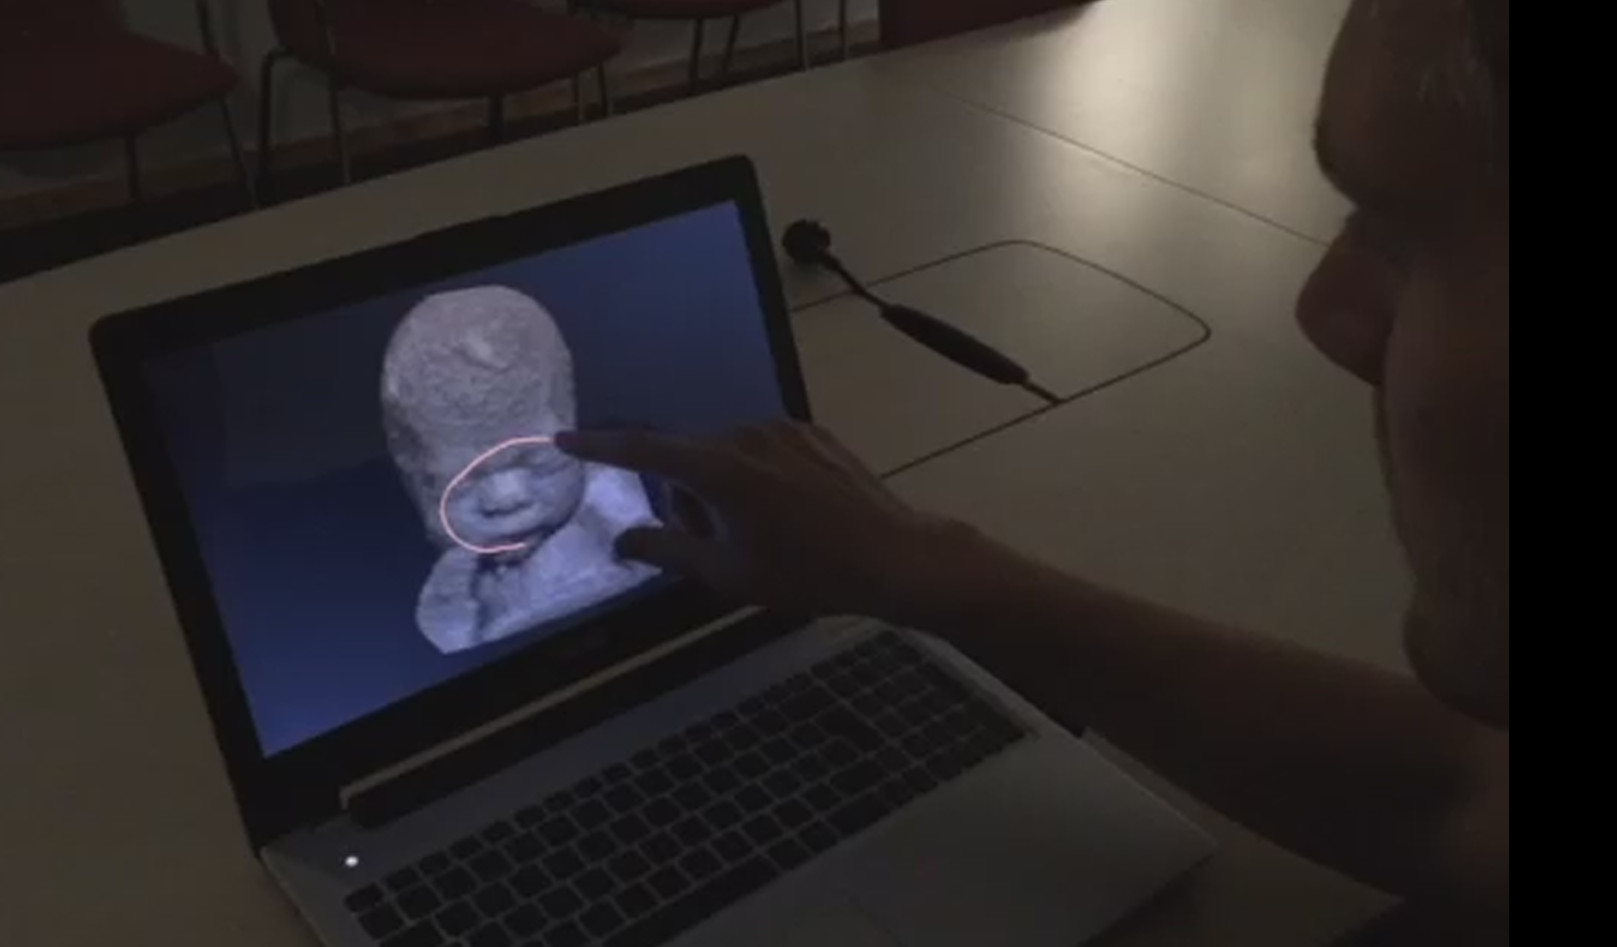
\includegraphics[width=1.0\linewidth]{images/touch_workstation}}
	\caption{Visualization of a fetus scanned using ultrasound. Touch screen interaction is used to change camera, transfer function and clipping.}
	\label{img:touch_workstation}
\end{figure}

\section{(Erik) Scenario: Exhibition Area}

In an exhibition area there is often both small to medium sized displays utilized to showcase and explore the scientific data. Furthermore, there is mostly none experience users and viewers present which interact and view others interact with the scientific data. There are a wide range of setups with certain displays and gadgets for immersive and exploratory purposes which can be utilized in an exhibition area, such as \cite{Laha:2013:VCB:2491367.2491368} (MORE REFS!!!). What they all have in common when it comes to these settings is that naturalness of the interaction is highly important. That fact, together with a reasonable level of functionality motivates the usage of hands-only setup, trough direct touch \cite{Klein:2012:DSD:2322389.2322403} and touchless methods \cite{O'hara:2013:NTP:2442106.2442111}.

In figure \ref{img:exhibition_table} we see an exhibition setup example, known as an autopsy table \cite{LRFPY11}, where data such as a CT scan of a human can be explored in a close to true scale environment, using direct touch and multi-touch gestures. In a sense it is just an increased version of a tablet, but suitable for a larger audience, as the area surrounding the table is significantly larger. With this in mind, the naturalness of the interaction for the user would benefit from as close to real life movements as possible, to support the true scale visualization. This is of course a challenge for direct touch displays, as there is a 2D instead of a 3D user experience. However, it can be considered a commonly known practice how to interact with touch displays, trough common gesture such as pinch and swipe.

\begin{figure}[htb]
	\centering
	\fbox{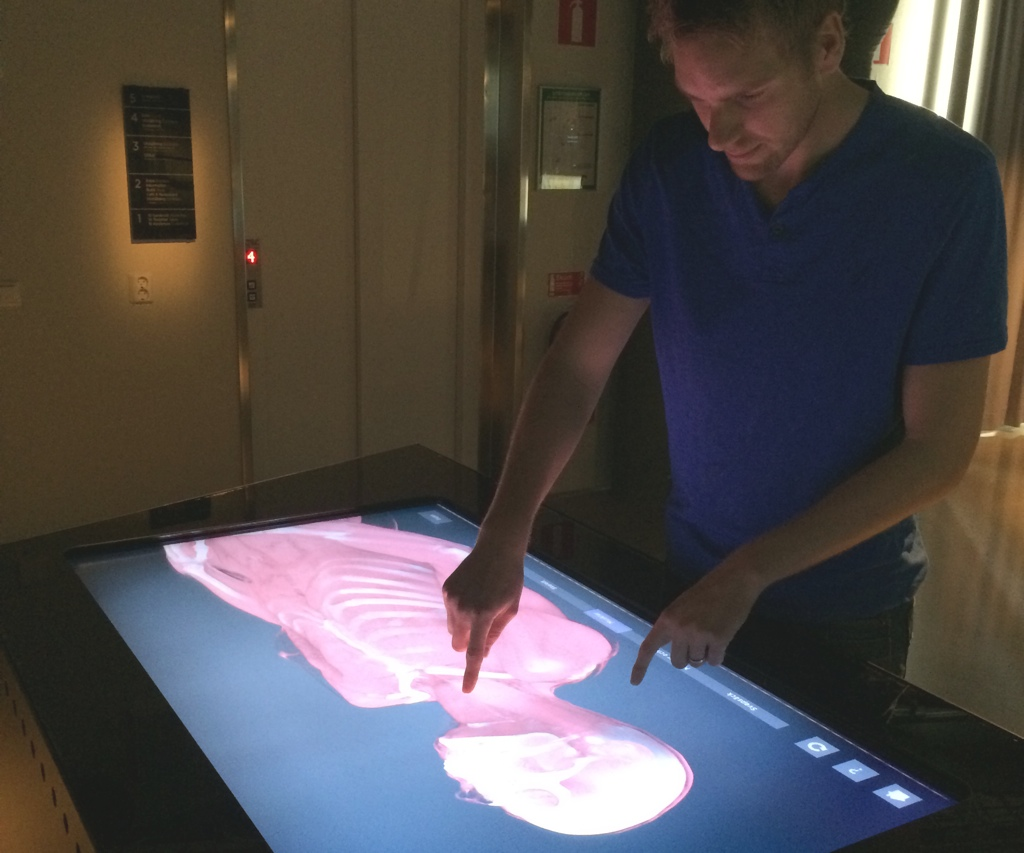
\includegraphics[width=1.0\linewidth]{images/exhib_table}}
	\caption{Exhibition: Touch Table}
	\label{img:exhibition_table}
\end{figure}

The setup seen in figure \ref{img:exhibition_kinect} is similar to figure \ref{img:exhibition_table} in terms of exploring data in true scale. The difference lie in the display surface, which is now without 2D interaction trough direct touch, and instead coupled with 3d interaction trough hand tracking. This setup can support a larger audience due the shear placement of the display surface, but comes with the downsides of a decoupled user interaction experience. The user will feel less in control of the data, even if you neglect the accuracy of the tracking, because he is not directly touching the display surface. Furthermore, the interaction might be less natural then direct touch, and the gestures more comprehensive to support the same level of functionality. As seen in figure \ref{img:exhibition_kinect}, a hand cursor is rendered which simulates the projection of the users hand onto the surface. Such visual cues not only help the user, but also allow a wider understanding for the audience to understand what operation the user is currently performing. Furthermore, the icons in the bottom are not only to avoid a more complex lineup of gestures for different operations, but also to make the operations performed more in contact with the visualization.

\textbf{Conclusions:}
Based on our observations we conclude that when performing a limited amount of operations, the setup with projector and 3D hand tracking is more optimal then the touch screen coupled with 2D finger gestures, when it comes to how the audience perceive the effect of interaction onto the visualization. The reason for this is that both the visualization and the projection of interaction can be visualized and perceived by the audience onto the display. This is not possible in practice if the user would directly interact with the display surface, as the projection of the users movement would be blocked by his hands, both for the audience and the user.

\begin{figure}[htb]
	\centering
	\fbox{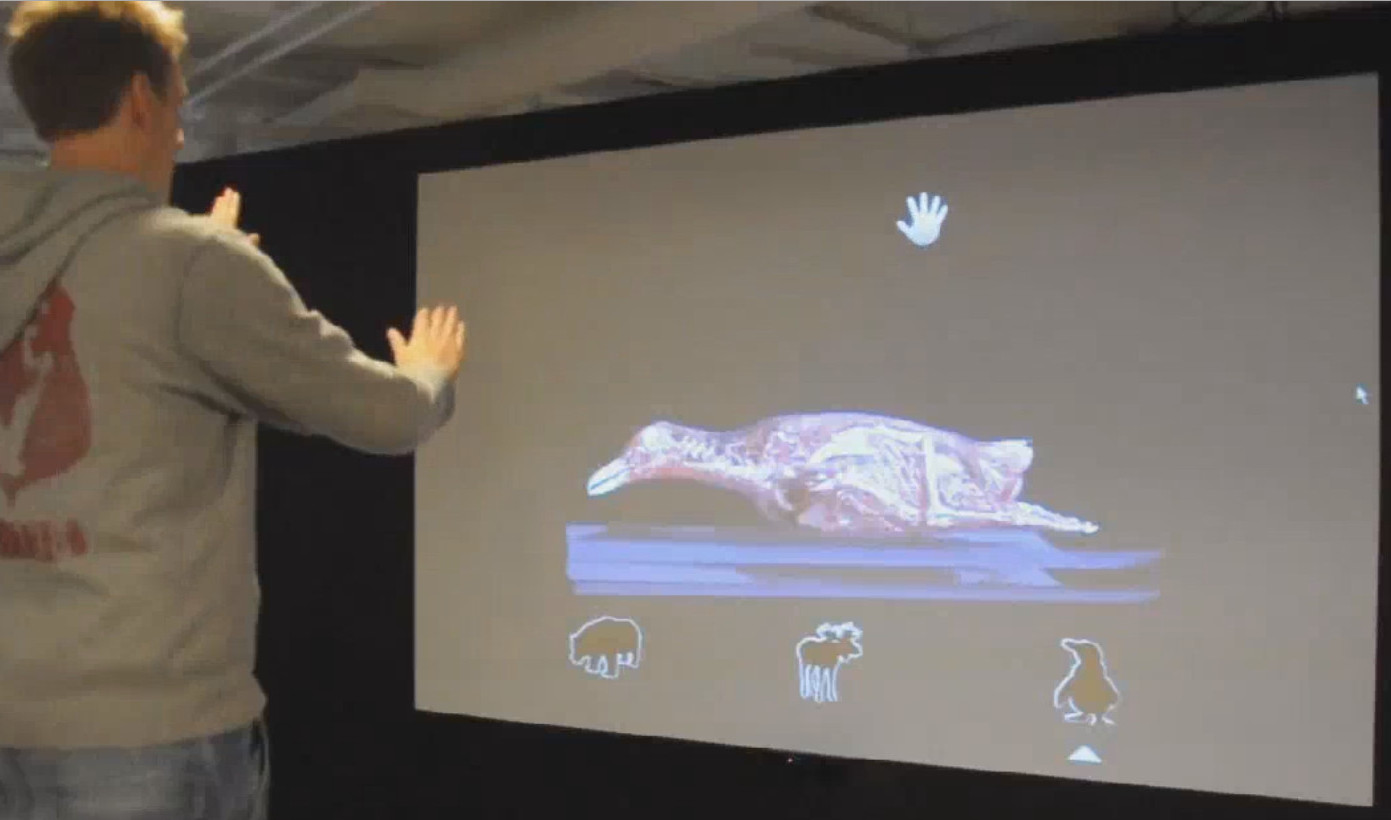
\includegraphics[width=1.0\linewidth]{images/exhib_rotate_peng}}
	\caption{Exhibition: Kinect, hand symbol supporting user and viewer guidance.}
	\label{img:exhibition_kinect}
\end{figure}

...

\section{(Alex) Scenario: Large Audience Presentation}

Oral Presentation
Being the most traditional form of 1 to many presentation techniques, oral presentations have been around since time immemorial.
While they were restricted to a lecturer talking to the audience in the beginning, over time more and more tools have been added to increase the information transfer to the audience.
Adding a blackboard allows the presenter to construct a visual representation of the information he is conveying.
In these early forms, the audience is witness to the construction and can follow the construction as it happens.
Note that there is a fundamental difference in learning between witnessing the creation vs observing the final result [citation needed].
Nowadays, the blackboard has been replaced with a whiteboard or alternatively a slide show, but the fundamental principle has not changed since the beginning.

A prime example of an enhanced oral presentation technique where the interaction technique matters is medical education based on cadavers.
Here, not only the content shown is of importance to the audience, but also the individual steps of how the presenter interacts with the body as this is one of the foci of study.
While the previous example supports in theory an unlimited size of audience, the medical example is limited by the fact that every audience member has to see the presenter and cadaver.
This is a good example of the [possible] trade-off between interaction design, audience size, and the possibility of using large-scale displays as a presentation tool.

The next logical development step from large-scale, large-audience displays is to include interactive content.
The results of the discussion for this scenario are independent of the data that is shown or the details of the interaction.
Principally, we can distinguish two classes of solutions for this interaction problem.
The first class, being direct interaction, requires the lecturer to perform the interaction himself.
For a detailed discussion of this class of solution, see below [or where ever].
The second class is indirect interaction [picture of Anders], where the lecturer is communicating orally with a second person controlling the content.
For this part, we assume that the audience hears the communication between the two people.
From an interaction point of view, this has both benefits and drawbacks.
One benefit is the added dynamics between the presenter and the controller, creating a more dynamic environment for the audience compared to just the presenter.
From an interaction point of view, the audience is witness to the intended action of the interaction, rather than the physical act of interacting.
The audience knows that, for example, the focus will be on a specific part of a rendering before it happens.
And rather than being witness of the manual interaction leading to that focus, it perceives the interaction as being completely indirect and decoupled from the presenter.
The explicit details of the interaction fall outside the regime of this paper, as the audience will not (in general) witness how the controller interacts with the visualization.
This decoupledness is the prime attribute for this class of solutions and whether this is a benefit or drawback depends on the situation to which it is applied.

A slight variant to this is the concept of remote presentations.
In this case the presenter is not in the same room as the intended audience, but his voice (and possible video) is streamed into the same room.
From an interaction point of view, this does not change much, as the presenter's interaction with the content was limited to a oral communication with the controller.
Furthermore, an increase in presence techniques, such as 3D conference applications will in the future further blur the line between a physically-present presenter and a remote presenter.


Dome vs VR Arena
In our research facility, we have access to two different display devices that bear superficial similarities, but induce fundamental differences in how the interaction with the audience works.

One of the display devices is a full field-of-view 160 degrees hemispherical dome with space for 99 audience members, which is projected using a stereo projector system.
This is a similar setup used in traditional planetariums, but in our case, an interactive rendering system is used instead to produce the content.
The interaction characteristics for this setup is that both the audience and the presenter are at a great physical distance (usually > 5 meter) from the projection surface.
This completely inhibits direct interaction techniques like pointing with a finger or doing gestures that are directly relate to the content that is shown on the screen.
Instead, indirect techniques must be used, like laser pointers, rendered cursors on the screen, gesture recognition, or oral communication with a controller.

The other setup available to us is a flat surface back-projection of three full HD projections which are aligned to produce a wide projection surface of about 5000x1080 pixel [check with Miro].
The room in which this is located seats about 30 people.
The benefit of having a back-projection is that the presenter can stand in front of the projection without casting a shadow on the projection surface, thus allowing physical access to the displayed content.
In comparison to the dome theater, this, and the limited size, allows the presenter to walk in front of the whole content and using natural gestures (which may be integrated, registered, and synchronized with the rendering) to interact with the content.
This natural, gesture-free interaction has been proved very useful in the workflow that we use in the facility.


Viewer(Audience) centered.

Presenter is always decoupled from the screen, as the presenter can not interact with the complete presentation surface. This is often due to the lack of touch capability, but foremost the sheer size of common screens for large audience presentations can not be reached from a standing location by the user.

Dome, movement, viewers benefit to see how presenter interacts with the data.
Thus, big 3D gestures better then gesture on touch device.

User should be standing in such away that the 3D movements the user performs can be projected correctly onto the screen.

Discuss interaction option made by audience, pros and cons

\begin{figure}[htb]
	\centering
	\fbox{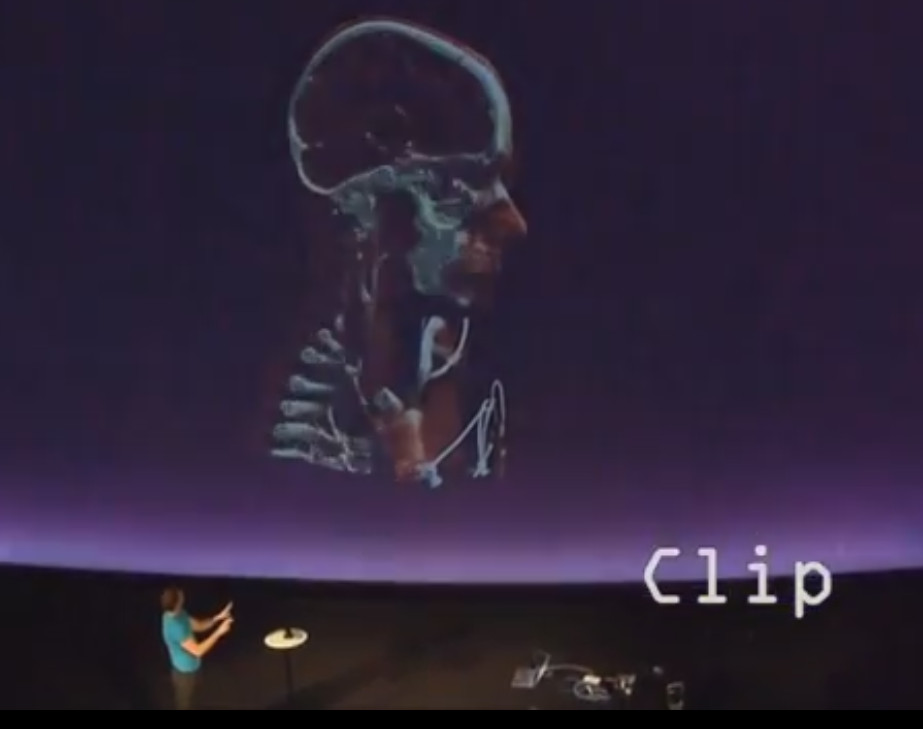
\includegraphics[width=1.0\linewidth]{images/dome_clip}}
	\caption{Dome}
	\label{img:dome_clip}
\end{figure}

\begin{figure}[htb]
	\centering
	\fbox{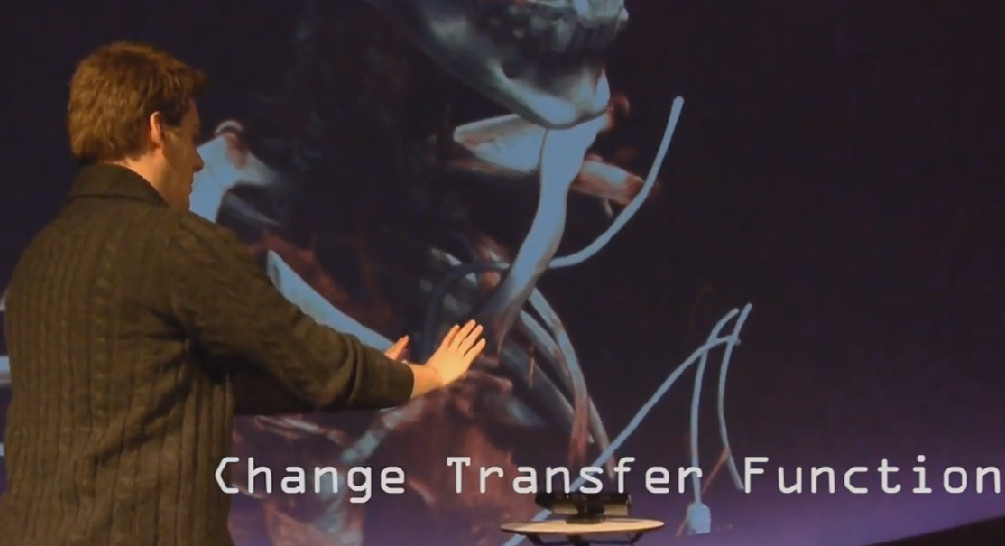
\includegraphics[width=1.0\linewidth]{images/dome_tf_change}}
	\caption{Dome Closeup}
	\label{img:dome_tf_change}
\end{figure}

\section{Conclusions}\label{sec:conclusion}

A decoupled interaction approach is always less intuitive then one which the viewing surface and interaction area is the same.

However, when a decoupled approach is necessary certain elements can be introduced in order to help the audience.

Such as projecting the hand onto the viewing surface.

\section{Future Evaluations of these scenarios}\label{sec:future}

Based on our observations we deem that an expansion of the research within viewer or audience centered interaction methods would be beneficial.

Within this subject, expert and none expert viewers have different ways of thinking and experiencing data exploration. Thus, the naturalness of the interaction could does be completely different for the different viewers.

\bibliographystyle{abbrv}
%%use following if all content of bibtex file should be shown
%\nocite{*}
\bibliography{literature}
\end{document}
